% !TEX spellcheck = en
%% document class file for the preparation of a paper
%% for the International Conference ICCAS 2007
%% global option 'fleqn' ensures equations flush left.
%% set '10pt' and 'twocolumn' options.

\documentclass[fleqn,10pt,twocolumn]{ICCAS2012}
\usepackage{amsmath}

%%%%%%% set heading and page number heare %%%%%%%%%%
%\setcounter{page}{101}
\begin{document}

\title{A $n$-dimensional Convex Hull Approach for Fault Detection and Mitigation for High Degree of Freedom Robots Humanoid Robots}

\author{Kevin Lynch${}^{1}$, Daniel M. Lofaro${}^{2}$ and Paul Oh${}^{3}$}

\affils{  	${}^{1}$Department of Computer Science, \\
		${}^{2}$Department of Electrical and Computer Engineering, \\
		${}^{3}$Department of Mechanical Engineering,\\
Drexel University, Philadelphia, PA, USA\\
kml43@cs.drexel.edu, dml46@drexel.edu, paul@coe.drexel.edu\\
        }
\thanks{*This project was supported by the Drexel Autonomous Systems Lab (DASL) and by a National Science Foundation - Partnerships for International Research and Education grant (\#0730206). \\ 
*Hubo was designed and created by our partner Dr. Jun-Ho Oh, Department of Mechanical Engineering, Korean Advanced Institute of Science and Technology, Daejeon, South Korea.}% <-this %

%\thanks{ \noindent
%   This paper is supported by my funding agencies.
%  }
\abstract{
\begin{center}
\large\bf{Abstract:}
\end{center}
\normalsize

\bf{
\noindent The degrees of freedom (DOF) of robots and complex systems have been increasing increasing exponentially since the early 20th century.
Today it is common place for complex control systems to have 40 DOF. 
This number is projected to be 70 DOF by the year 2020.
Robots with high DOF allows for complex tasks such as tool manipulation, greater human-robot interaction and agile full-body locomotion.
More DOF require greater attention to local communication delays, bandwidth, system configuration and stability.
In addition different tasks being performed by separate parts of the robot in tandem bring on greater issues including controller timing and priorities.
The increase in DOF on single system requires that the traditional methods of controller design be re-examined.

\noindent This dissertation describes a Unified Algorithmic Framework for High Degree of Freedom Complex Systems and Humanoid Robots that allows a user to develop controllers using a three tier infrastructure.
The Unified Algorithmic Framework called Hubo-Ach is a multi-process based system that allows for robust multi-rate simultaneous control and seamless implementation between virtual, miniature, and full-size robots with no modification.
The three tier infrastructure provides different levels of cost to entry and testing.
Examples of this field tested framework functioning on simulated, miniature, and full-size high DOF robots is given as well as validation by external researchers.
}




}

\keywords{
    Humanoid Robotics, Fault Detection, Error Mitigation, $n$-dimensional Convex Hull
}

\maketitle

%-----------------------------------------------------------------------
The number of degrees of freedom (DOF) of control systems are increasing exponentially since the early 20$^{th}$ century.
Today it is common place for complex control systems to have 40 DOF. 
This number is projected to be 70 DOF by the year 2020 (see Section~\ref{sec:numdof}).
\textit{The increase in DOF on single system requires that the traditional methods of controller design needs to be re-examined}.
High DOF complex system, or robots, allow for complex tasks such as using human tools and interfaces \cite{lofaroRAM2013,lofaroTePRA2013HuboAch,lofaroTePRA2013Valve,gtechIK}, playing music \cite{lofaroEURASIP2011, 6094987,lofaroIASTED2011,5686847} and other complex tasks \cite{lofaroHumanoids2012,lofaroGamesRobot,tepraLadder2013}.

\cite{orocos-gadeyne-ijrr2005}
\cite{multiPC-arch-1185243}
\cite{multi-thread-robot-5602743}
\cite{multi-thread-snake-1541141}
\cite{multi-thread-5524083}
\cite{openHRP}
\cite{Webots}




Due to the nature of these highly redundant complex electrical mechanical system it is common to have multiple different controllers running in tandem.  
Different controllers are needed when the system is in different states or doing different tasks or performing multiple tasks at the same time.
Combining these controllers is a problem in complex system.
This problem is hard when each controller has different frequencies, timing requirements (asyncronous vs. syncronous), latency restrictions, newest state data ie smore important then older state data and most basic of all languages the controller is written in.
This is especially true for complete and complex autonomous systems.
I define a complete and complex autonomous system as an electro mechanical mechanism with high degree of freedom (DOF) that is capable of making its own decisions through the use of sensor data processed by its artificial intelligence (AI).
The combination of high DOF and the requirement for autonomy makes the work space broad and controllers complex.
The overarching question becomes; What is the control system structure for a complete and complex autonomous systems with high DOF, a multitude of sensors, AI performing high-level and low-level tasks all while keeping a stable system structure conducive to collaborative work?
Current methods of solving the problem of controller synchrony and latest state data is to keep your critical control elements in the primary control loop.
Inter-process communication (IPC) and/or network sockets to communicate between the high level and low level processes even if written in different languages.
The majority of IPC have the problem of \textit{head of line} blocking (HOL) which means you must read the older data in a buffer before you read the newest data.
In the computer science field this is not a problem because all data being intact is typically desired.  
In the field of robotics and control the most recent state data is more important to a real-time control system to act on.
This thesis shows that by expanding on the idea of multi-process controllers connected to high-speed low-latency IPC you can create a \textit{robot layer} on a computer platform that will allow low-level controllers to run in separate processes while still allowing them access to the most recent data as the priority.
The new technical idea is the \textit{robot layer}, a control layer that allows external processes to run like normal and not deal with the specifics of the given robot system.
The robot system can be replaced by a simulated system without any of the processes needing to be modified or even know of the change.
This allows more mature controllers to be easily interfaced with this system without modifying control rates or timing.
This \textit{robot layer} must be:
\begin{itemize}
\item Have a IPC latency much less then that of the robot's inherent sampling period $t_{ipc}<<T_{r}$
\item Allow for command rates much slower then the inherent sampling period $T_{slow}>>T_{r}$
\item Allow for command rates much faster then the inherent sampling period $T_{fast}<<T_{r}$
\item Allow for arbitrary command rates.
\item Allow for real-time and non-real-time controllers to command actuators
\item Allow for all processes to have access to the newest data first
\item Allow for no more then one rt time step delay between command and robot actuator retrieval
\item Commanded such that it is for an arbitrary robotic actuator.
\item Triggering for process synchronization
\item Triggering for simulator synchronization and holding
\end{itemize}
We can succeed now not only because the bleeding edge technology allows for the fast enough communication between processes with access to the latest data.

Results are measured quantitatively and qualitatively.
Data showing proper loop rates, timings, controller implementation, simulation connections etc. show the viability of the system.
User survey shows methodology is sound, useful, and practical.





My Thesis shows is that a multi-process control structure coupled with the proper timing mechanisms is conducive to answering these questions.
It is shown with physical experiments and the creation of Hubo-Ach\cite{lofaroRAM2013}; a fully functional Sim-Time and Real-Time control system for complete and complex autonomous systems.

Through experimentation I prove my control system is a viable way of controlling complete and complex autonomous system and still be conducive to collaborative work.  
A road map of how my research has taken me to my thesis is shown in Section~\ref{sec:roadmap}.
As proof of viability I show the basic structure of my system \textit{Hubo-Ach} in Section~\ref{sec:hubo-ach}.  
I give step by step examples in Section~\ref{sec:simpleExamples}.
Section~\ref{sec:simulator} shows how we can move from real-time to using a simulated version of the platform in simulation time without having to change the controller.
Section~\ref{sec:task} describes the experiment which consists of making the robot preform an advanced task that pulls together visual, kinematic, path planning and other controllers together using this one system.
The techniques used stem from my contributions in Section~\ref{sec:contributions}.
Section~\ref{sec:results} shows the results of the experiment thus show the viability of the system.
Lastly Section~\ref{sec:conclusion} discusses the results of the work and the future of this system.

Before I continue it is important to note that my work has already been validated by my pears because:
\begin{itemize}
\item It was chosen to be the primary control system for the DARPA Robotics Challenge Track-A Team DRC-Hubo, Section~\ref{sec:drc}.
\item It is being used in the NSF-MIRR project\footnote{NSF-MIRR: Major Research Infrastructure Recovery and Reinvestment (MIRR) \#CNS-0960061 sponsored by the the U.S. National Science Foundation (NSF)}.
\item It is currently being used by MIT, WPI, Purdue, Ohio State, Swarthmore College, Georgia Tech, and Drexel University.
\end{itemize}

For the remainder of this document the complete and complex autonomous systems that I will be referring to are robots.
The majority of examples given will be in reference to humanoid robotics and the Hubo2+ (KHR-4+) platform.
The Hubo platform is described in Section~\ref{sec:hubo}.






The idea for a Control Archetecture for High Degree of Freedom Complex Systems stems from a gap in physical implimentation of control algerithms for robot hardware.

The simplest approach to developing robot software is to intergrate all functionality in one program.  
This functionality includes the following controllers:
\begin{itemize}
\item Hardware Control
\item Perception
\item Planning
\item Kinimatics
\item etc.
\end{itemize}

If all of this functionality is in one process then it has the bennifit of freedom of inter process comunication latency.
However being in one process also means that if one of the controllers laggs or faults it cause the entire controller to lag or fault.
This is of great concern if a non-prority controller such as vision processing faults causing a priority controller such as a ballance controller, to fail.
This will cause the robot to fall.
How is this fixed?
One solution and my proposed solution is to use inter-process comunicatoin (IPC).
Inter-process comunication is a method of exchanging data between multiple processies.
Typical POSIX methods (cite here) give you the \textbf{oldest} information first and have locks on the memroy when processies are writing to it.
Robots work in the physical world. 
More recent information is more important to it then older.
In most cases it is acceptiable to know the most recent data and never read any of the older data.
This would happen if your sensors update at a faster rate then that of the robot.
Typically robot actuiators have a bandwidth much much lower then that of a mondern conputer.
If sensor informatio is shared using traditional shared memory over POSIX methods the controller would have to read the older information before it reaches the information it is most interested in, the newest data.
This is called head of line blocking (look up).

It is desired to make a multi-process controller that can share data between multiple processies with low-latency and no head of line blocking.
There are a few IPCs that offer no head of line blocking and low-latency.  
After much research (inserte examples here) it was found that the Ach IPC wuld best fit my needs.




\section{Methodology}\label{sec:methodology}
%\subsection{Balance and Stability}\label{sec:sec:balance}
Each of the methods used have to be stable through the motion in order for the system to be stable (i.e. not to fall down).  
The well known zero-moment-point (ZMP) criteria is what each method must adhere to in order to stay statically stable\cite{Vukobratovic19721}.  
To handle perturbation an active balance controller was added.  
The active balance controller is applied on top of the pre-defined trajectories.  
Hubo is modeled as a single inverted pendulum with the center of mass (COM) located at length $L$ from the ankle.  
The compliance of the robot is composed of a spring $K$ and a damper $C$, see Fig.~\ref{fig:invPen}.  
An IMU located at the COM gives the measured orientation.

\begin{figure}[t]
  \centering
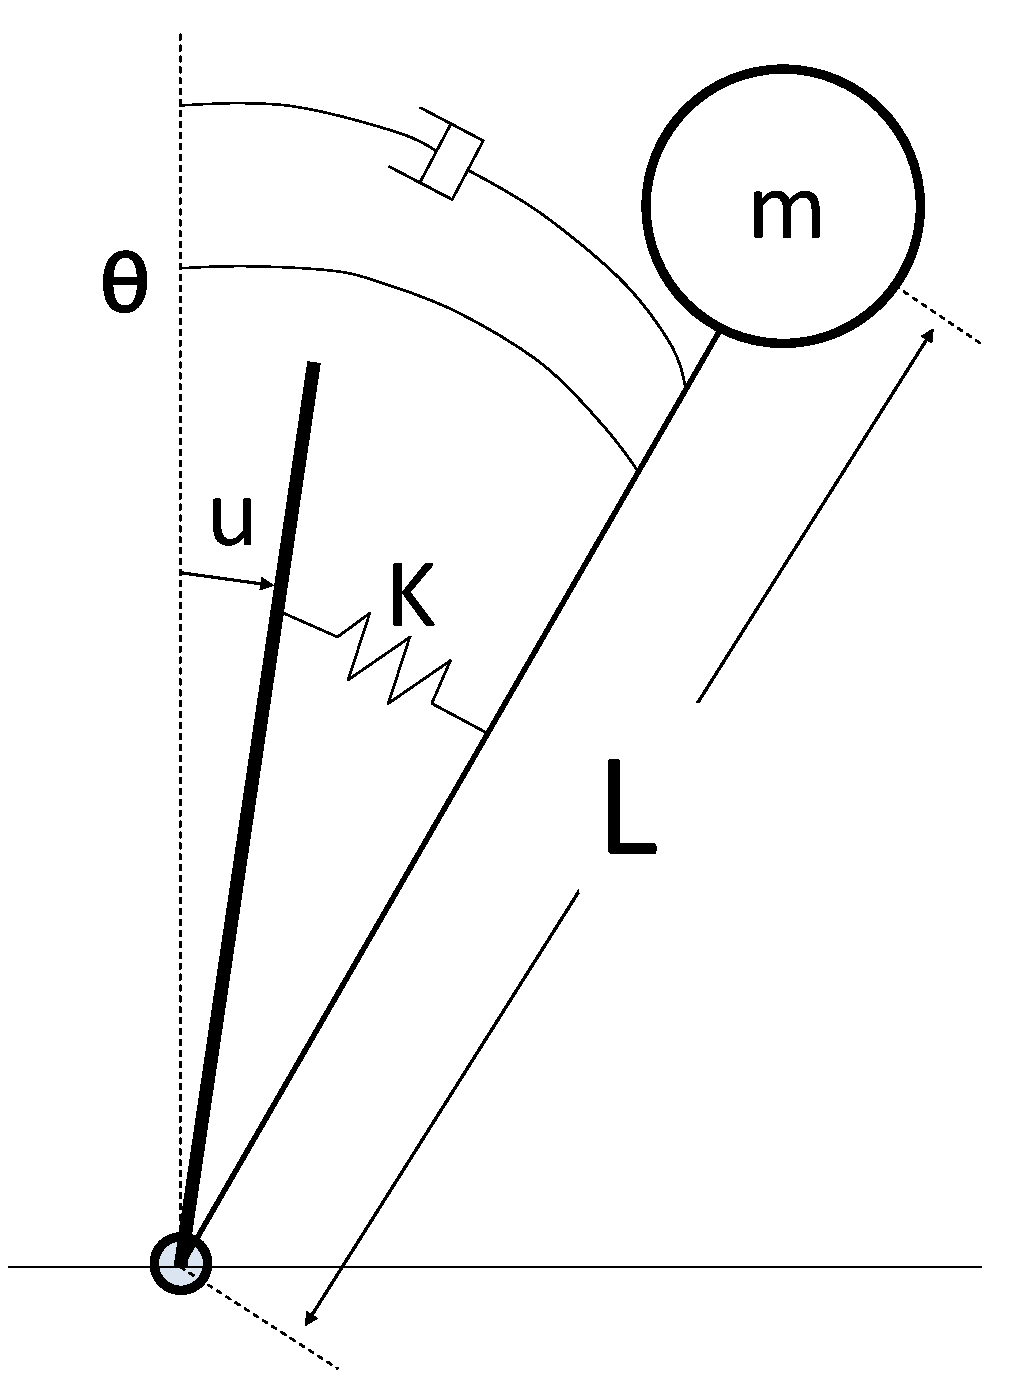
\includegraphics[width=0.4\columnwidth]{./pix/invPen3.pdf}
  \caption{Hubo modeled as a single inverted pendulum with COM located a distance $L$ from }
  \label{fig:invPen}
\end{figure}

The dynamic equation of the simplified model is assumed to be the same in both the sagittal and coronal plane.

\begin{equation}
mL^2\ddot{\theta}+C\dot{\theta}-K\theta = Ku
\end{equation}

This can be linearized and made into the transfer function:

\begin{equation}
%G(s) = \frac{\Theta(s)}{U(s)} = \frac{K}{ mL^2s^2 + Cs + (K - mgL)}
G(s) = \frac{\Theta(s)}{U(s)} = \frac{\frac{K}{mL^2}}{s^2+\frac{C}{mL^2}s + \frac{K-mgL}{mL^2}}
\end{equation}

Prior work on the model and controller for the Hubo by Cho et. al. calculated K=753 $\frac{Nm}{rad}$ and C=18 $\frac{Nm}{sec}$ using the free vibration response method\cite{5379574}.


\begin{figure}[ht]
  \centering
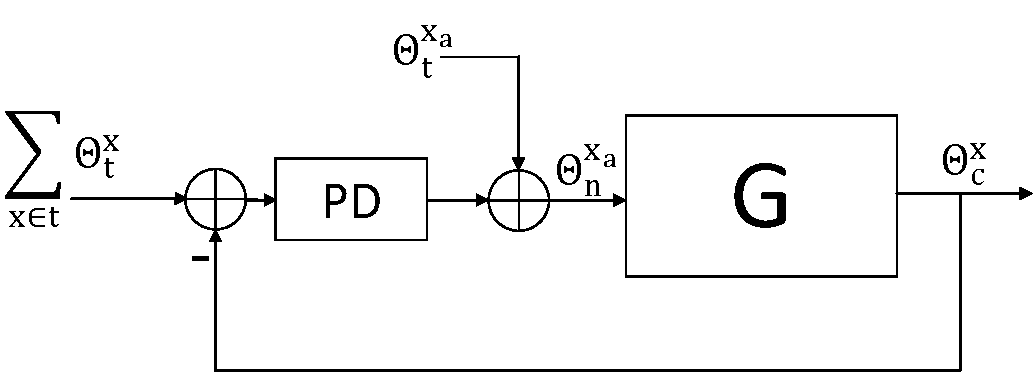
\includegraphics[width=0.8\columnwidth]{./pix/blockDiagram3.pdf}
  \caption{Block diagram of the balance controller used to balance Hubo in this work.}
  \label{fig:ctrlBlockDiagram}
\end{figure}

The control law is as follows
%ffFor the ankle roll (in the coronal plane) it is always assumed that the desired orientation of the COM is zero degrees.  Thus the roll of the IMU is taken as the error.

\begin{equation}
\theta_n^{x_a} = \theta_t^{x_a} + \left(K_p^x+sK_d^x\right)\left(\sum\limits_{x \in t} \theta_{t}^x - \theta_{c}^x\right)
%\theta_{n}^x = \theta_{t}^x + \left(K_p^x+sK_d^x\right)\left(\sum \theta_{t}^x - \theta_{c}^x\right)
%\theta_{n}^x = \theta_{t}^x + (K_p^x+sK_d^x)(\sum \theta_{t}^x - \theta_{c}^x)
%\theta_{new} = \theta_{traj} + (K_p+sK_d)(\sum \theta_{leg} - \theta_{IMU})
\end{equation}

Where $\theta_t$ is the desired trajectory of the lower body (pitch or roll), $x$ denotes pitch or roll and $x_a$ denotes pitch or roll on the ankle.  $\theta_{c}$ is the orientation of the center of mass in the global frame.  $\theta_n$ is the resulting trajectory.  $K_p$ and $K_d$ are the proportional and derivative gains.  The resulting control allows for a stable stance even with perturbations from upper body motions.



\section{Expected Results}
\label{sec:expResults}

It is expected that the recorded metrics will converge and give us a well defined convex hull for normal operating state.  Failure states such as ZMP loss or  actuator over current is also expected to create a well defined hull due to it's tight correlation with the kinematics and sensor data.  Failures that are not tightly correlated other metrics, such as actuator zero or actuator status, are not expected to form a well defined hull.  Similar to the software system it is expected that the mitigation methods will very from platform to platform despite having the same faults present.

\section{Conclusion}
Through the failure at the Philadelphia Convention Center it has been shown that there is a need for fault state detection and mitigation.
It has been shown that Aniketos system is capable of creating an $n$-dimensional convex hull describing proper running states and failure states on software system.  A plan has been described to apply Aniketos to a physical platform which included injecting faults into the physical system and creating the convex hull from the recorded sensor and state data.  The expected results are described in Section~\ref{sec:expResults} and are based on the results from the software testing.

%\subsection{Faults}
\label{sec:faults}
The states that we will be analyzing for the creation of the convex hull for
the fault detection mapping fall into four categories, faults, status, low
level feedback, high level feedback.  A list of the


%Electro-mechanical systems inevitably fail during use.  Failures during
operation typically cause system halts.  This is particularly hazardous to
robots that require feedback to balance such as biped humanoid robots.  For
biped humanoids these errors typically include, but are not limited to,
actuator failure due to over torque or loss of zero-moment-point
(ZMP) \cite{zmp35} causing a robot fall or collapse.  This is exceptionally
harmful to adult size humanoid robots due to their weight.  It is key for the
robot to recognize when it is entering a failure state and be able move to a
safe running state.  This paper focuses on way of automatically detecting when
a failure is about to occur and choosing the proper mitigation technique.

Current methods of mitigation of ZMP loss for biped humanoids been investigated
by Kiyoshi Fujiwara et al. \cite{4115653}.  These methods involve finding an
optimal falling trajectory that reduces the instantaneous force of the robot at
impact by creating multiple impact stages\cite{4399327}.  This method was fully
tested on an HRP-2FX (HRP-2P surrogate) and partially on an HRP-2P.  This work
did not include a method of determining a falling state, it is assumed that a
fall is in progress.  Additional work on detecting a fall and reducing fall
damage has been shown by Kunihiro Ogata et al.\cite{4755950}.  An active
shock-reducing motion reduces the impact damage by following the center of
gravity (COG) and attempting to keep it close to the ZMP support polygon.  The
falling state is determined when the predicted ZMP departs from the support
polygon. This method was tested on a miniature humanoid robot.  Additional work
on determining a fall state using machine learning techniques\cite{4813885}.
Reimund Renner et al. used parameter estimation of multiple sensors to detect a
falling state\cite{4058847}.

These methods are able to detect a specific fault state, however a need of
detecting different fault states requires more general methods.  These methods
must include monitoring not only sensor data but also actuator failure status.



%%%%%%%%%%%%%%%%% BIBLIOGRAPHY IN THE LaTeX file !!!!! %%%%%%%%%%%%%%%%%%%%%%
%%---------------------------------------------------------------------------%%
%
%\begin{thebibliography}{99}


%\bibliographystyle{plain}
%\bibliography{mit}

\bibliographystyle{IEEEtran}
%\bibliographystyle{plain}
\bibliography{mit}{}


%\end{thebibliography}

%
%%--------------------------------------------------------------------%%

\end{document}
